\documentclass[12pt]{article}

\usepackage{fullpage}
\usepackage{graphicx, rotating, booktabs} 
\usepackage{times} 
\usepackage{natbib} 
\usepackage{indentfirst} 
\usepackage{setspace}
\usepackage{grffile} 
\usepackage{hyperref}
\usepackage{adjustbox}
\setcitestyle{aysep{}}


\singlespace
\title{
\textbf{Testing the Public Goods Theory of Alliances}
	}
\author{Joshua Alley\footnote{Graduate Student,
Department of Political Science, Texas A\&M University.}}
\date{{\normalsize \today}}

\bibliographystyle{apsr}

\begin{document}

\maketitle 

\doublespace



%----------------------------------
\section{Introduction}



\citet{OlsonZeckhauser1966} argue that international alliances are subject to a collective action problem. 
Smaller alliance participants ``free ride'' on the contributions of larger members. 
This claim is intuitive and influential. 


As of November 2018, Olson and Zeckhauser's article has been cited 1670 times.
Furthermore, they claim alliances are exemplars of collective action in international organizations. 
Given its salience and broad implications, this public goods theory of alliances merits careful scrutiny. 


But 52 years after the publication of ``An Economic Theory of Alliances,'' we have limited evidence for or against free-riding in alliances. 
The lack of solid evidence is the result of two research design issues. 
First, many empirical models are unidentified.
Second, the overwhelming majority of tests focus on NATO. 


Olson and Zeckhauser's approach to measuring the defense burden and state size creates an identification problem. 
They estimated a correlation between military spending as a share of national income on national income, and has been widely emulated. 
This approach places GDP on both sides of the equation, so the models are unidentified.


Ratio dependent variables such as military expenditures as a share of GDP often lead to spurious results \citep{Kronmal1993}. 
In Olson and Zeckhauser's test, changes in GDP impact the independent and dependent variable. 
There is a deterministic component to the relationship between GDP and the ratio of military expenditures to GDP. 


\citet{PluemperNeumayer2015} address the identification problem by examining changes in spending among NATO members. 
In their framework, unresponsiveness to US and Soviet military spending is evidence of free riding among non-US NATO members.
They find no correlation between the size of a NATO member and free-riding, which they argue contradicts Olson and Zeckhauser. 
However, they do not include the United States in their sample, which omits a crucial data point for testing the size argument.\footnote{Given the focus on responses to US spending, this decision is understandable.}


% So what is the problem here? 
Despite the canonical status of \citet{OlsonZeckhauser1966}, their predictions have not been subjected to a general, well-identified test. 
The majority of free-riding tests focus on NATO, and we can conclude NATO members spend less on the military thanks to allied capability \citep{PluemperNeumayer2015, GeorgeSandler2017}.
But NATO is only one case. 


% by the way, it's mostly NATO
We do not know whether the public goods theory of alliances applies beyond NATO. 
My survey of the literature on alliance participation and military spending found six tests of the public goods theory of alliances outside of NATO. 
All six of those studies include GDP in the independent and dependent variable, creating an identification problem. 


% So it total, there's a lot we don't know
Due to identification problems and emphasis on NATO, we have no evidence for the generalizability of the public goods theory of alliances. 
Understanding NATO is worthwhile. 
But it is insufficient to assess the value of the public goods theory of alliances. 


% Why we should care
Failure to test the public goods theory of alliances well has two important consequences. 
First, it hinders the accumulation of knowledge. 
Without a valid and comprehensive test, the explanatory of the public goods theory of alliances is unclear. 


% Why we should care: policy and free riding
Second, the public goods theory of alliances has an outsized impact on policy debates. 
The idea of free-riding is ubiquitous in popular and policy debates. 
If the public goods theory of alliances makes inaccurate predictions, charges of free-riding should be reassessed.


% I'm not the first one to address this theory: first comprehensive empirical evidence
Other scholars have questioned the public goods theory of alliances on theoretical grounds \citep{Palmer1990, SandlerHartley2001}.  
But such theoretical revisions are premature without knowledge that a more parsimonious public goods model is inappropriate. 
This paper provides the first comprehensive test of the public goods theory of alliances.  


Establishing the empirical validity of the public goods theory of alliances is crucial for academic theory and policy debates. 
Below, I outline two possible solutions to this challenge. 
Both examine the role of alliance participant size in multiple alliances from 1816 to 2007. 


The first approach uses a conventional panel data research design, with an aggregate measure of alliance participation. 
In this model, I examine whether small states reduce military expenditures as a result of increasing allied spending, and if that effect is diminishing in state size. 
The second design employs a Bayesian model to estimate the association between treaty contribution and member's military spending for every alliance. 
Neither design finds evidence to match Olson and Zeckhauser's predictions. 


The paper proceeds as follows.
First, I summarize the public goods theory of alliances and generate two testable predictions.
Then, I describe the results of a panel-data test of the first prediction.
The third section tests the second prediction with a multilevel model. 
The final section assesses aggregate support for the public goods logic, as well as implications for scholarship and policy. 


\section{The Public Goods Theory of Alliances}

% this needs to be succint- aim for 500 words. 

% summarize argument
Why are alliances subject to a public goods problem? 
The aggregate capability of an alliance provides security for members. 
Because a treaty cannot exclude members without undermining its purpose, security is a public good. 


Individual members gain security from treaty participation, regardless of their individual contribution. 
Olson and Zeckhauser expect that larger members of the alliance with bear a higher defense burden, because these states value defense from the alliance more. 
Smaller alliance members free-ride on the contributions of larger partners. 


% Develop implications for test: one for each section. 
There are two implications of this argument. 
First, large and small states should respond differently to changes in allied military spending. 
If Olson and Zeckhauser's argument is correct, smaller states should decrease military spending in response to greater allied military spending. 
Larger states will be less responsive to increased allied spending. 
This implies a conditional relationship between allied spending, state size, and state military spending. 


\begin{quote}
\textsc{Hypothesis 1}: The marginal effect of allied spending on state military spending will be negative for small states, and increasing in state size. 
\end{quote}


The other prediction addresses individual alliance treaties. 
If larger states bear a disproportionate share of the alliance burden, then within each alliance, increasing contribution will lead to higher military spending. 
States that contribute more to the alliance will increase military expenditures to maintain the output from the treaty. 


\begin{quote}
\textsc{Hypothesis 2}: Within alliances, increasing treaty contribution will be positively associated with military spending. 
\end{quote}


Alliances where we observe a positive correlation between treaty contribution and military spending conform to Olson and Zeckhauser's expectations. 
No correlation indicates larger members are not increasing military expenditures.
A negative correlation between treaty contribution and military spending implies larger members decrease spending. 


I now test these two predictions from the public goods theory of alliances in a sample of all states except microstates from 1816 to 2007.\footnote{Including states with really small GDP values makes estimating the interactions in Section 2 difficult.}
The next section examines Hypothesis 1 by interacting changes in total allied spending and GDP.
This approach aggregates multiple treaties into a single measure of alliance participation. 


\section{Testing Hypothesis 1}

To examine Hypothesis 1, I rely on conventional measures of state size and alliance participation. 
Olson and Zeckhauser use GDP as a proxy for state size, and I employ the Maddison project's data to construct a measure of GDP \citep{Boltetal2018}. 
Total allied capability is a common measure of alliance participation \citep{Sorokin1994, MorganPalmer2003}. 
I measure total allied capability as the military spending of all defensive or offensive alliance partners of a state \citep{Leedsetal2002}. 


The dependent variable is changes in the natural log of military spending \citep{SingerCINC1988}. The log-level of military spending is non-stationary.
Modeling the DV in levels might lead to spurious inferences. 


Because Hypothesis 1 implies a conditional relationship, I interact allied spending and GDP in the following regression model:

\begin{equation} 
y = \beta_1 + \beta_2 \mbox{GDP} + \beta_3 \mbox{Ally Spend} + \beta_4 \mbox{GDP} \times \mbox{Ally Spend} + \beta X + \epsilon
\end{equation}


$\beta_2$ and $\beta_3$ are the constituent terms and $X$ is a matrix of control variables with coefficient vector $\beta$.
Hypothesis 1 implies $\beta_2$ should be positive, and $\beta_3$ should be negative. 
The interaction term $\beta_4$ should be positive. 


I estimate this model with a robust regression estimator. 
Even after the log transformation, military spending produces heavy-tailed residuals, making OLS inefficient \citep{RaineyBaissa2018}. 
Robust regression re-weights observations using the size of the residual, making it less sensitive to large deviations than OLS. 


In the robust regression, I control for several correlates of alliance participation and military spending. 
First, I include the lagged level of spending, because larger military budgets can produce greater changes in spending. 
I control for international war \citep{Reiteretal2016}, civil war participation \citep{SarkeesWayman2010}, and a count of annual MIDs \citep{Gibleretal2016}. 
Other controls address salient alliance characteristics, including average democracy and number of members across a state's alliance treaties.   
Last, I control for regime type, external threat \citep{LeedsSavun2007}, and Cold War years. 


\subsection{Results}


Estimates from this model do not match the expectations of Hypothesis 1. 
\autoref{tab:rreg-res} summarizes results from the robust regression estimator. 
As expected, GDP is positively correlated with military spending. 
Changes in allied spending have no effect on military spending, however. 
The interaction term of changes in allied spending and GDP is also statistically insignificant. 

\begin{table}[ht]
\centering
\begin{tabular}{lrrr}
  \hline
 & Value & Std. Error & t value \\ 
  \hline
	Change Allied Spending & -0.020 & 0.044 & -0.453 \\ 
	ln(GDP) & 0.012 & 0.002 & 6.161 \\ 
	Change Allied Spending $\times$ ln(GDP) & 0.001 & 0.002 & 0.805 \\ 
  Lag ln(Military Spend.) & 0.992 & 0.001 & 805.703 \\ 
  Avg Alliance Size & 0.001 & 0.000 & 4.370 \\ 
  Avg Alliance Democracy & -0.001 & 0.001 & -1.547 \\ 
  International War & 0.090 & 0.010 & 9.396 \\ 
  Civil War Participation & 0.005 & 0.007 & 0.717 \\ 
  Polity & -0.000 & 0.000 & -0.777 \\ 
  International Threat & 0.026 & 0.011 & 2.437 \\ 
  Cold War & 0.046 & 0.004 & 11.472 \\
	Constant & -0.180 & 0.038 & -4.690 \\ 
   \hline
\end{tabular}
\caption{Robust Regression Estimates: Allied Spending, GDP, and changes in military spending 1816-2007. A t-value greater than two implies statistical significance at conventional levels (p < .05).}
\label{tab:rreg-res}
\end{table}


I cannot conclusively infer the absence of an interaction from the coefficients alone \citep{BramborClarkGolder2006}. 
\autoref{fig:abs-margins-plot} plots the marginal effect of allied military spending across the distribution of GDP. 
The marginal effect of allied military spending is never negative. 
There is no conditional relationship between state size and changes in allied spending. 

\begin{figure}
	\centering
		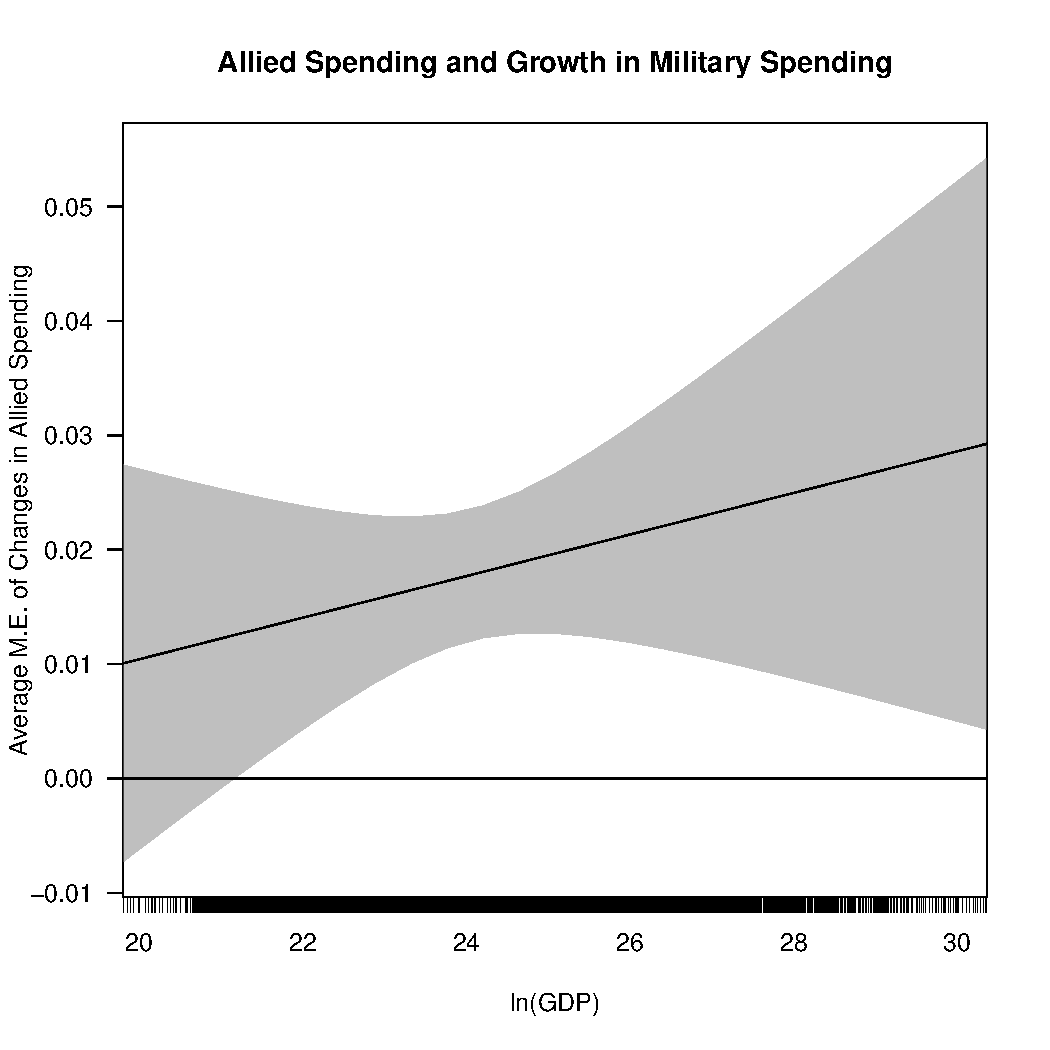
\includegraphics[width=0.95\textwidth]{abs-margins-plot.pdf}
	\label{fig:abs-margins-plot}
	\caption{Average Marginal Effect of increasing allied military spending on a state's military spending, across the range of GDP.}
\end{figure}


These results hold if I replace robust regression with OLS estimator or employ kernel estimation of the interactive relationship \citep{Hainmuelleretal2017}.\footnote{See the Supplementary files.} 
I also estimated a model that treats states with an alliance as the estimation sample, and used the Heckman two-stage estimator to address non-random selection into alliances. 


It is possible that by aggregating multiple alliance treaties into a single measure, this model does not capture heterogeneous effects of individual treaties.
Small states can make a large contribution to an alliance if their partner is even smaller. 
So the next section examines how many alliances match the expectations of the public goods theory. 


\section{Testing Hypothesis 2}


Testing Hypothesis 2 requires estimating the association between alliance contribution and military spending for each alliance.
For each of the 285 alliances that promise military support,\footnote{ATOP offensive and defensive treaties.} I estimate a parameter measuring the impact of increasing alliance contribution on military expenditures. 
Bayesian estimation regularizes estimates with hundreds of parameters, so I fit the following model using STAN \citep{Carpenteretal2016}.

The full model starts with state-year changes in the natural log of military spending $y_{it}$.
I model the DV with a t-distribution to account for heavy tails.
$\nu$ is the degrees of freedom parameter--- as $\nu$ increases, the t distribution becomes more like a normal distribution. 


\begin{equation}
y_{it} \sim student_t(\nu, \mu, \sigma) 
\end{equation}


Most of this model follows standard panel data designs.
The expected value of the outcome $\mu_{it}$ depends on a constant $\alpha$, state and year varying intercepts $\alpha^{st}$ and $\alpha^{yr}$, a lagged DV $y_{t-1}$, and control variables $X_{it} \beta$. 
In this specification, I include all controls besides the alliance portfolio averages from the first robust regression in $X$.


\begin{equation}
\mu_{it} = \alpha + \alpha^{st} + \alpha^{yr} + \eta y_{it-1} + X_{it} \beta + Z_{it} \lambda 
\end{equation}


The $Z_{it} \lambda$ term captures the impact of multiple alliances. 
$Z$ is a matrix of state participation in alliances--- columns are alliances, rows are state-year observations. 
If a state is not in an alliance, the corresponding element of the matrix is equal to zero. 
If a state is part of an alliance, the corresponding element of the matrix is equal to a state's military spending as a share of allied spending. 
The alliance contribution elements of the matrix range from 0 to 1, because some states have no military spending.\footnote{Costa Rica is the best-known example of a state with no military spending.} 


$\lambda$ is a vector of 285 alliance-specific parameters.  
Because $Z$ contains alliance contribution, these parameters capture the association between treaty contribution and military spending. 
A positive $\lambda$ implies that as contribution to the alliance increases, members spend more. 


When a state is not in an alliance, the corresponding $\lambda$ is multiplied by zero, and has no impact. 
Alliance participation only affects military expenditures if a state contributes. 
Each alliance a state is a member of has a separate impact on military spending.
Thus, each alliance estimate holds the impact of other treaties constant.     


\subsection{Results} 


If the public goods theory of alliances is correct, we should observe many positive $\lambda$ parameters. 
Because I employed Bayesian modeling, each $\lambda$ has a posterior distribution.\footnote{See the appendix for a full summary of priors, convergence and model fit.} 
I focus interpretation on the posterior mean and 90\% credible intervals.\footnote{I use the 90\% credible intervals because inferences around the 95\% intervals can be less stable.}
The posterior mean is the expected value of $\lambda$, while the credible intervals capture uncertainty around that estimate.  


\begin{figure}[htbp]
	\centering
		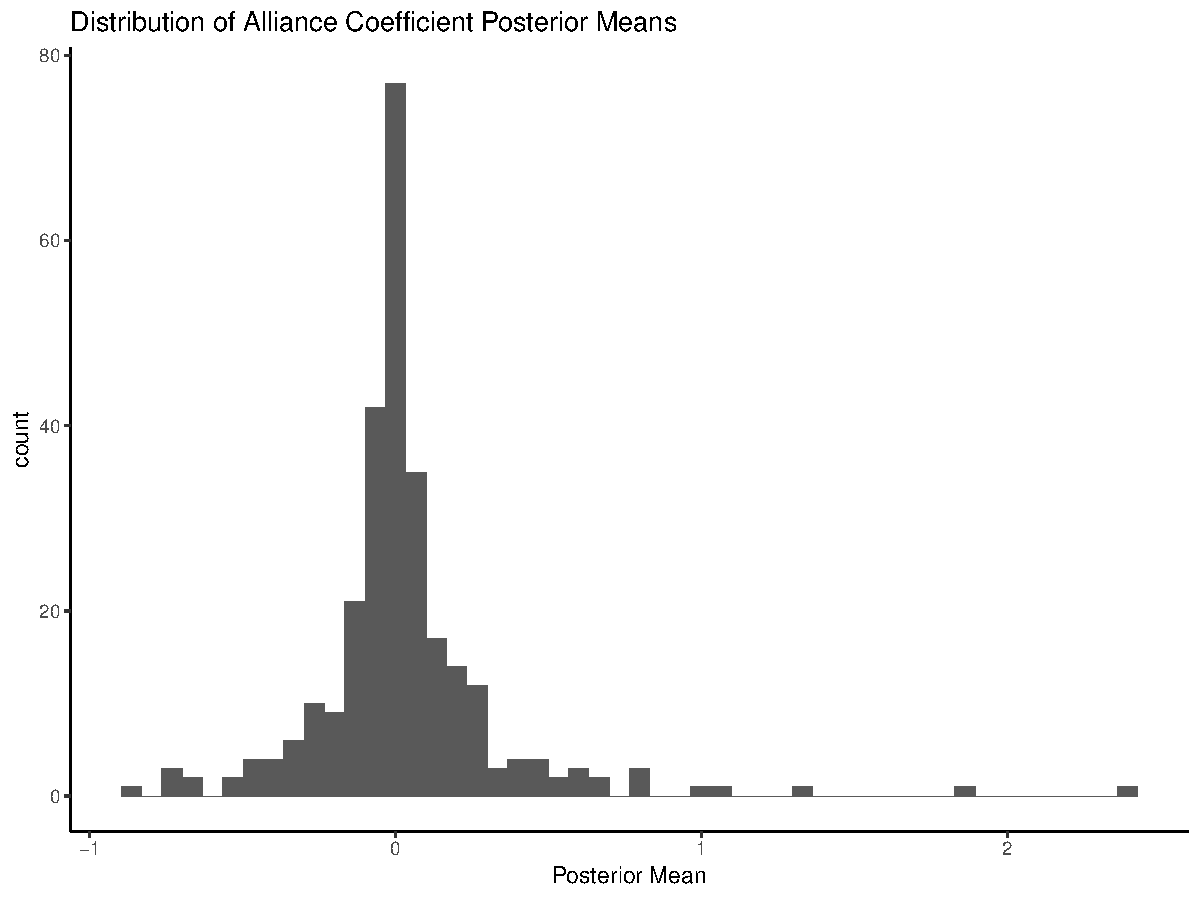
\includegraphics[width=0.95\textwidth]{alliance-coefs-hist.pdf}
	\caption{Posterior mean of association between alliance contribution and military spending in 285 defensive and offensive alliances from 1816 to 2007.}
	\label{fig:alliance-coefs-hist}
\end{figure}


\autoref{fig:alliance-coefs-hist} summarizes the posterior mean of the 285 alliance coefficients. 
Most posterior means are close to zero. 
There are large positive values, but also a good number of large negative values.


141 of 285 alliances have a positive posterior mean. 
144 of 285 alliances have a negative posterior mean. 
The large number of negative values is some evidence against Hypothesis 2. 
However, the posterior means do not convey whether the impact of increasing alliance contribution can be distinguished from zero. 


\autoref{fig:alliance-coefs-year} plots the $\lambda$ parameter for each alliance against the start year of the treaty.
Points mark the posterior mean. 
The error bars encapsulate the 90\% credible interval.\footnote{The credible intervals summarize the 5\% and 95\% quantiles of the posterior.}  


\begin{figure}[htbp]
	\centering
		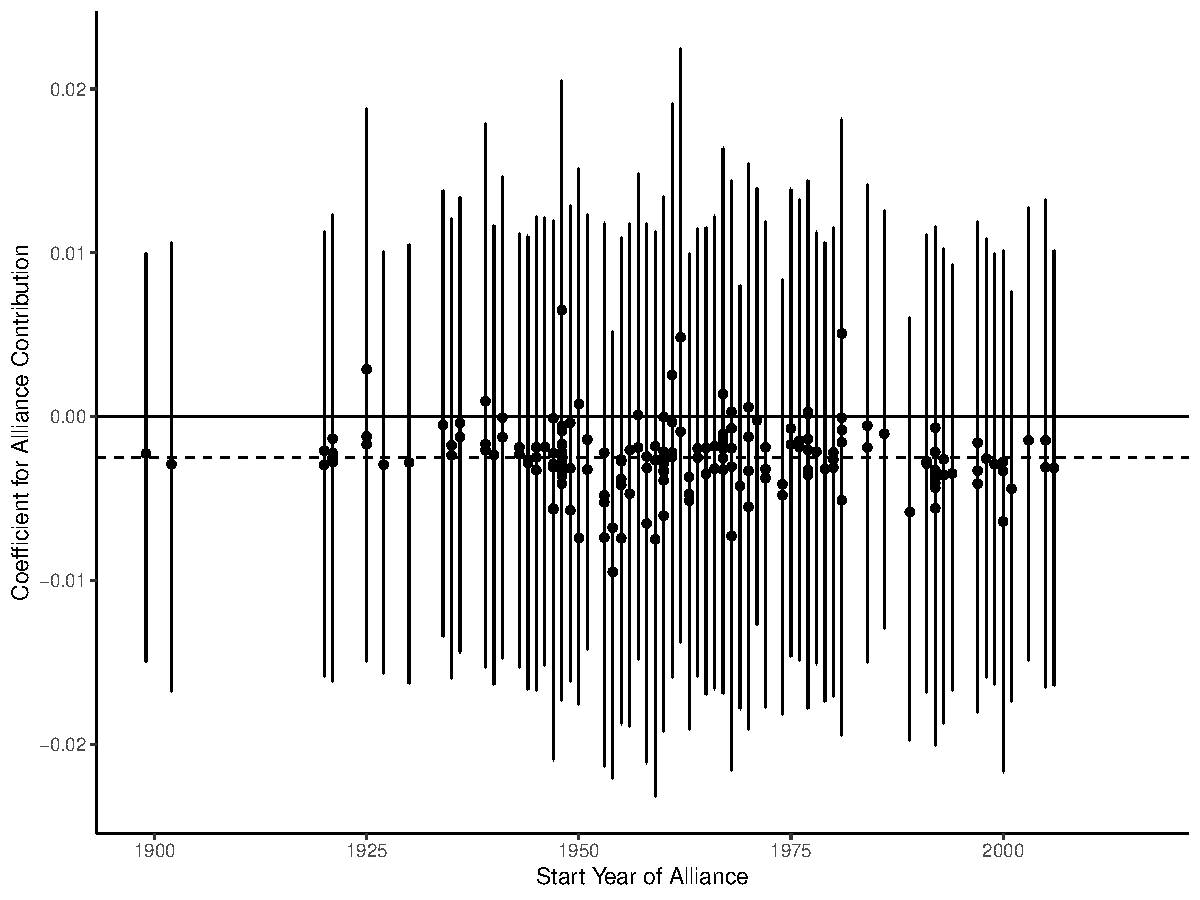
\includegraphics[width=0.95\textwidth]{alliance-coefs-year.pdf}
	\caption{Estimated association between alliance contribution and defense spending in 285 defensive and offensive alliances from 1816 to 2007. Points represent the posterior mean and the error bars cover the 90\% credible interval.}
	\label{fig:alliance-coefs-year}
\end{figure}


Most posterior means are close to zero, so 251 credible intervals include zero. 
There are 20 alliances where the credible interval includes only positive values. 
That leaves 14 treaties where the credible interval covers only negative values. 


20 of 285, or 7\%, is a dismal prediction success rate for Hypothesis 2. 
There is no association between treaty contribution and military spending in most alliances.
The 14 negative $\lambda$ parameters imply larger members of those alliances \emph{spend less} on the military, which the public goods theory cannot explain. 


Alliances with a non-zero $\lambda$ provide additional information. 
We can look at these alliances to assess the potential role of free-riding. 
In \autoref{fig:nonzero-alliance-coefs}, I plot the posterior means of $\lambda$ for all 34 alliances.  
Several of these alliances have a large expected impact on military spending. 


\begin{figure}
	\centering
		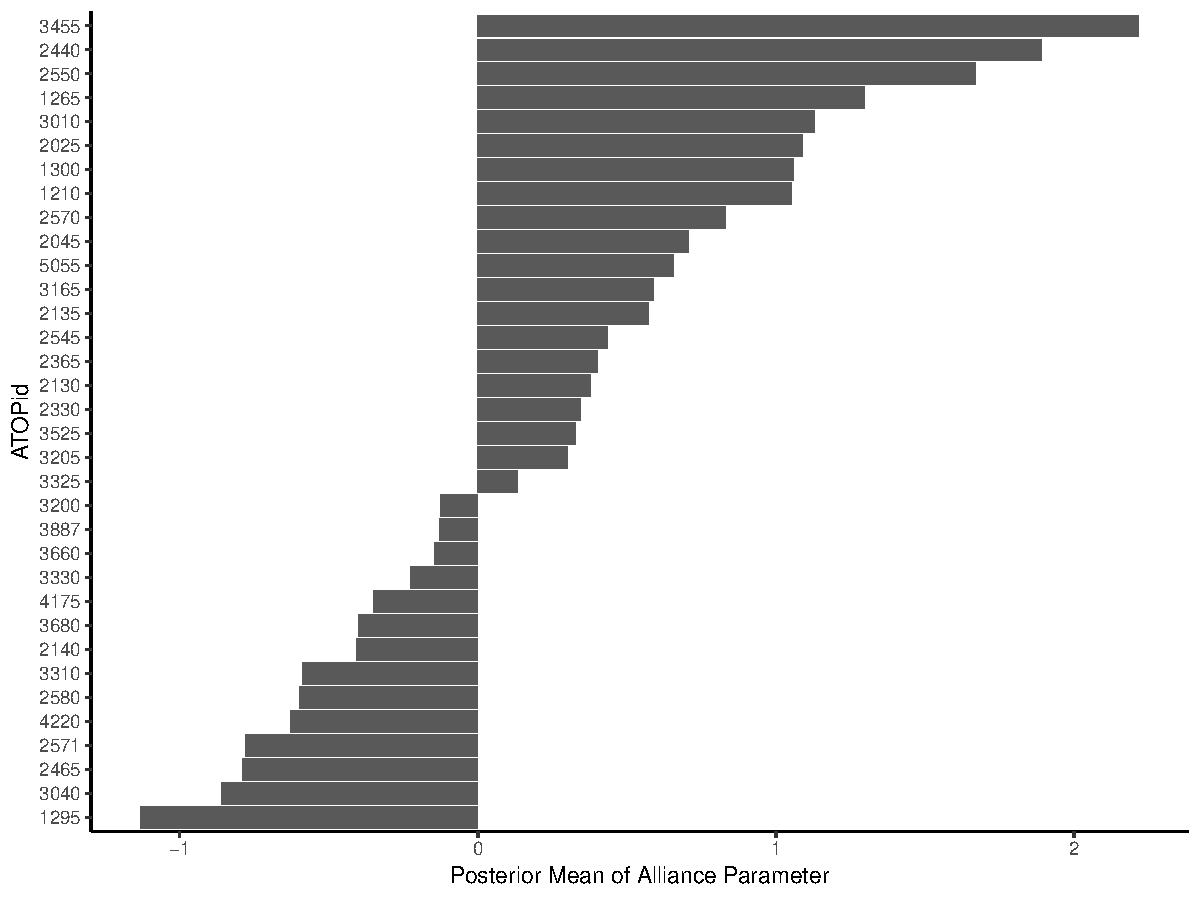
\includegraphics[width=0.95\textwidth]{nonzero-alliance-coefs.pdf}
	\caption{Bar plot of $\lambda$ for alliances where treaty contribution is positively or negatively correlated with military spending. The Y axis is the ATOP project's alliance identifier.}	
	\label{fig:nonzero-alliance-coefs}
\end{figure}


The largest positive association between treaty contribution and military spending is the 1961 Defense Pact of the African and Malagasy Union (ATOPID 3455). 
The second largest is a 1939 defense pact between the UK and Poland (ATOPID 2440). 
The third largest is the Allied Coalition during World War II (ATOPID 2550). 


Two of these three cases are not obvious examples of free-riding. 
Any increase in British spending in 1939 reflects the elevated risk of war from the Polish treaty.  
This and the Allies of World War II are a special cases in Olson and Zeckhauser's model where defense spending is a superior good--- increases in income are spent on defense. 
These treaties expanded the obligations of their larger members, requiring increased defense spending. 


The negative $\lambda$ parameters reflect alliances with little resemblance to a public goods model. 
The largest negative association is an 1870 alliance between Prussia and the UK, signed during the Franco-Prussian war (ATOPID 1295). 
This treaty provided for the neutrality of Belgium, allowing the British to reduce defense spending. 
The second largest negative $\lambda$ is tied to ATOPID 3040--- a 1946 treaty between the UK and Jordan, where the latter agreed to assist British forces in the region. 
Last, the third largest negative $\lambda$ is a June 1939 alliance between France and Turkey aimed at securing the Mediterranean (ATOPID 2465). 


These three negative cases suggest that overstretched large states can use alliances to secure their interests and reduce spending. 
Without treaties with Prussia and Jordan, the UK would have spent more to defend Belgium in 1870 and hold its Middle Eastern possessions in 1946. 
France used the 1939 treaty with Turkey for similar purposes. 
These alliances structure particular exchanges among members, rather than provide some public good. 


NATO is the best example of collective defense, where a public goods model might apply. 
The estimated $\lambda$ for NATO offers no support for the public goods theory of alliances, however. 
The posterior mean is $-0.004$, and the credible interval ranges from -.26 to .26.  
Greater contribution to NATO is unassociated with military spending. 
This finding corroborates the results of \citet{PluemperNeumayer2015}. 


Other alliances may be subject to free-riding. 
ATOP alliance \#3010 is a possible case. 
This treaty was an Inter-American Hemispheric defense pact during World War II--- other American states may have been content to rely on the United States. 
The 2006 African Union Non-Aggression and Common Defense Pact (ATOPID 5055) also has a positive $\lambda$ that might be explained by free-riding.  


This second set of estimates provides little support for predictions from the public goods theory of alliances. 
In 88\% of alliances, there is no association between treaty contribution and military spending. 
Even cases where treaty contribution is positively correlated with spending may not reflect collective action problems. 


\section{Conclusion}

% Add paragraph summarizing results
Taking the results from testing Hypothesis 1 and 2 together, there is little evidence for the predictions of the public goods theory of alliances. 
There is no conditional relationship between GDP and changes in allied spending.
Moreover, there is no association between treaty contribution and military spending in most alliances. 


These findings should increase our skepticism about the public goods model of alliances. 
Although Olson and Zeckhauser's model is simple and intuitive, it lacks explanatory power. 
Better identified empirical models and examination of multiple treaties shows little evidence small states leave larger counterparts to bear a higher burden. 


My results reinforce extant theoretical skepticism about the public goods model. 
\citet{Palmer1990} and \citet{SandlerHartley2001} provide two theoretical critiques that merit further scrutiny. 
Constructing parsimonious models of alliances and defense effort is the next challenge for scholars. 
Components of the public goods model and these alternatives may provide a useful starting point. 


Some of the results raise additional questions for theoretical work. 
Why do we observe 14 alliances where increasing alliance contributions are associated with reduced spending?
Why is the effect of greater allied spending mostly positive in Model 1? 
Derivatives of the public goods theory may struggle to address these questions. 


Furthermore, scholars should reassess the idea of ``free-riding'' in alliance politics. 
Free-riding is inextricable from a public goods understanding of alliances.
But if key predictions of the public goods model have little empirical support, free-riding is an inaccurate description of reduced defense effort by alliance participants.  
Charges of free-riding are normatively loaded and may mask exchange between alliance members \citep{Lanoszka2015}. 


We should not abandon the public goods model in international politics more generally. 
The public goods model may apply to other international organizations. 
Inferring collective action problems in other international organizations from alliances is inappropriate, however. 


The public goods model of alliances should have a less salient role in discussions of alliance participation and defense effort. 
I find little evidence that reduced military spending by alliance members is the result of a collective action problem. 
A pure public goods models has little explanatory power in alliance politics. 



\singlespace


%\bibliography{C:/Users/jkalley14/Dropbox/Research/MasterBibliography}  
\bibliography{C:/Users/Josh/Dropbox/Research/MasterBibliography} 





\end{document}

